%\section*{Summary}
%
%\begin{itemize}
%\item SPDHG excellent alg for non-smooth priors, but only sinogram
%\item modern TOF PET data is extremly sparse (Figure) -> SPDHG inefficient
%      in terms of memory and speed
%\item LM projections are much faster than sino projections for usual count levels
%      (Table)
%\item propose LM-SPDHG that solves both issues
%\item 1st step: better init
%\item 2nd step: rewrite SPDHG in terms of LM updates
%\end{itemize}

%%%%%%%%%%%%%%%%%%%%%%%%%%%%%%%%%%%%%%%%%%%%%%%%%%%%%%%%%%%%%%%%%%%%%%%%%%%%%%%%%%%%%%%%%%%%%%%%%%%%%%%%
%%%%%%%%%%%%%%%%%%%%%%%%%%%%%%%%%%%%%%%%%%%%%%%%%%%%%%%%%%%%%%%%%%%%%%%%%%%%%%%%%%%%%%%%%%%%%%%%%%%%%%%%
%%%%%%%%%%%%%%%%%%%%%%%%%%%%%%%%%%%%%%%%%%%%%%%%%%%%%%%%%%%%%%%%%%%%%%%%%%%%%%%%%%%%%%%%%%%%%%%%%%%%%%%%
%%%%%%%%%%%%%%%%%%%%%%%%%%%%%%%%%%%%%%%%%%%%%%%%%%%%%%%%%%%%%%%%%%%%%%%%%%%%%%%%%%%%%%%%%%%%%%%%%%%%%%%%

\section{Introduction}

A major challenges of image reconstruction in positron emission tomography (PET)
is noise suppression since the acquired emission data suffer from high levels of Poisson
noise due to limitations in acquisition time, injectable dose and scanner sensitivity.
To limit the transfer of the data noise into the image during model-based iterative
reconstruction (MBIR), different strategies exist. 
One possibility is to add a ``smoothing'' prior to the data fidelity term in the cost
function that is being optimized.
In general, we can write the optimization problem for PET image reconstruction as
%
\begin{equation}
\argmin _{x\geq 0} \sum_{i=1}^{m} \underbrace{(Px + s)_i -  d_i \log \left( (Px + s)_i \right)}_{D_i(x)} + \, \beta R(Kx),
\label{eq:primal}
\end{equation}
%
where $x$ is the PET image to be reconstructed, $P$ is the (TOF) forward model including the effects
of attenuation and normalization and blurring, $d$ are the acquired prompt TOF coincidences 
(the emission sinogram), and $s$ are additive contaminations including random and 
scattered coincidences. 
$\sum_{i=1}^m D_i(x)$ is the negative Poisson log-likelihood, $i$ is the index of the data (TOF sinogram)bin and $m$ is the total number of data (TOF sinogram) bins.
$R(Kx)$ is the ``smoothing prior'' consisting of a generic linear operator $K$ that calculates 
local differences and a proper, convex, lower-semicontinous function $R$.
The level of regularization is controlled by the non-negative scalar factor $\beta$.
A specific example for $K$ would be the gradient operator $\nabla$, e.g. approximated by finite forward 
differences in the discretized setting.
Using the gradient operator for $K$ and the mixed L2-L1 norm for $R$ leads to the well-known 
Total Variation (TV) prior \cite{Rudin1992}.

Unfortunately, many advanced smoothing priors aiming for edge-preservation 
such as e.g. TV \cite{Rudin1992}, Total Generalized Variation (TGV) 
\cite{Bredies2010}, Joint T(G)V \cite{Rigie2015,Knoll2016}
Parallel Level Sets \cite{Ehrhardt2016a,Schramm2017} or directional Total Variation (DTV)
\cite{Ehrhardt2016} use non-smmoth functions for $R$ which permits the use of simple and efficient 
purely gradient-based optimization algorithms to solve \eqref{eq:primal}.

Using the fact that $D = \sum_i D_i$ and $R$ are equal to their convex biconjugates 
$D^{**} = \sup_y \langle Px + s, y \rangle - \sum_{i=1}^{m} D_i^*(y_i)$ 
and $R^{**} = \sup_w \langle Kx, w \rangle - R^*(w)$, respectively,
we can rewrite \eqref{eq:primal} as the saddle point problem
%
\begin{equation}
\argmin _{x\geq 0} \, \sup_{y,w} \,  \langle Px + s, y \rangle + \langle Kx, w \rangle - \sum_{i=1}^{m} D_i^*(y_i) - \beta R^*(w/\beta) ,
\label{eq:saddle}
\end{equation}
%
introducing the dual variables $y$ and $w$ and the convex dual of the Poisson log-likelihood given by
%
\begin{equation}
D_i^*(y_i) =
\begin{cases}
-d_i + d_i \log \left( \frac{d_i}{1-y_i} \right) & \text{if } y_i < 1 \\
\infty & \text{else} \ .
\end{cases}
\end{equation}
%
Problem \eqref{eq:saddle}, can be efficiently solve using the generic primal-dual hybrid gradient (PDHG) 
algorithm by Chambolle and Pock \cite{Chambolle2011} even for non-smooth priors.
PDHG is in iterative algorithm that requires the evaluation of the complete forward and adjoint operator
in every update.
The usage of the original PDHG algorithm to solve \eqref{eq:saddle} for real-world state-of-the-art
TOF PET systems usually means extremly long computation times, because evaluation of $P$ (corrected TOF 
forward projection) and $P^T$ (corrected TOF back projection) 
for state-of-the-art TOF PET systems are usually slow and because several hundreds to thousand of updatesare needed to obtain reasonable convergence.

To overcome this limitatation, Chambolle et al. published a stochastic extension of PDHG called SPDHG 
for saddle point problems that are separable in the dual variable \cite{Chambolle2018} in 2018.
In contrast to PDHG, SPDHG has the advantage that the complete forward and adjoint operator is 
split into $n$ subsets and that in every update only a random subset of the forward
and adjoint operator chosen according to probability $p_k$ have to be evaluated.
In \cite{Ehrhardt2019}, Ehrhardt et al. applied SPDHG to 3D non-TOF PET reconstruction with TV-like
priors and could indeed show that around 10 complete projections and back projections are sufficient 
to obtain reasonable convergence using SPDHG with 252 subsets.
Moreover, the authors also demonstrated that preconditioning further accelerates convergence.
The resulting SPDHG algorithm to solve \eqref{eq:saddle} is summarized in Algorithm \ref{alg:spdhg},
where the proximal operator of the convex conjugate of the negative Poisson log-likehood $D_i^*$ 
is given by
%
\begin{equation}
(\prox_{D_i^*}^{S}(y))_i = \frac{1}{2} \left(y_i + 1 - \sqrt{ (y_i-1)^2 + 4 S_i d_i} \right) \ .
\label{eq:proxD}
\end{equation} 
%
The proximal operator for $R^*$, obviously depends on choice of $R$ but can be efficiently 
computed using point-wise operations for many popular choices of $R$.
As mentioned in \cite{Ehrhardt2019}, Algorithm \ref{alg:spdhg} converges if we use the preconditioned
step sizes
%
\[ S_k = \gamma \, \text{diag}(\frac{\rho}{P_k 1} )\qquad  T_k = \gamma^{-1} \text{diag}(\frac{\rho p_k}{P^T_k 1}) \ , \]
% 
and
%
\[ S_{n+1} = \gamma \, \frac{\rho}{\|K\|} \qquad T_{n+1} = \gamma^{-1} \frac{p_i\rho}{\|K\|} \ , \]
%
setting $T = \min_{k=1,\ldots,n+1} T_i$ pointwise, and choosing $\rho<1$ and $\gamma>0$.

%
%
%
%
%
\begin{algorithm}[t]
\begin{algorithmic}[1]
\small
\State \textbf{Initialize} $x(=0),y(=0),(w=0)$, $(S_i)_i,T,(p_i)_i$,
\State $\overline{z} = z = P^T y + K^T w$
\Repeat
	\State $x = \proj_{\geq 0} (x - T \overline{z})$
	\State Select $i \in \{ 1,\ldots,n+1\} $ randomly according to $(p_i)_i$
  \If{$i \leq n$}
	\State $y_i^+ \gets \prox_{D_i^*}^{S_i} ( y_i + S_i  ( P_i x + s_i))$
	\State $\delta z \gets P_i^T (y_i^+ - y_i)$
	\State $y_i \gets y_i^+$
  \Else
	\State $w^+ \gets \beta \prox_{R^*}^{S_i/\beta} ((w + S_i  K x)/\beta)$
	\State $\delta z \gets K^T (w^+ - w)$
	\State $w \gets w^+$
  \EndIf
	\State $z \gets z + \delta z$
	\State $\overline{z} \gets  z + (\delta z/p_i)$
\Until{stopping criterion fulfilled}
\State \Return{$x$}
%\EndFunction
\end{algorithmic}
\caption{SPDHG for PET reconstruction \cite{Ehrhardt2019}}
\label{alg:spdhg}
\end{algorithm}
%
%
%

\subsection{Problem}

\section{Materials and Methods}

\subsection{Better intialization of sinogram SPDHG}

Use quick EM-TV (e.g. 1 iteration 28 susbets) as initializtion for $x$.
Initialize $y$ (dual variable of data) as
\begin{equation}
y^0 = 1 - \frac{d}{Px^0 + s} \ .
\end{equation}
Note that this also means that the initial y is 1 in bins where we have
no data such that we don't need to keep y in memory during the iterations.

(optionally) intialize $w$ (dual of gradient) in subgradient of $R(Kx^0)$



%-----------------------------------------------------------------------------
\begin{algorithm}[t]
\begin{algorithmic}[1]
\small
\State \textbf{Input} event list $N$
\State \textbf{Calculate} event counts $\mu_e$ for each e in $N$ (see text)
\State \textbf{Split} event list $N$ into $m$ sublists $N_i$
\State \textbf{Initialize} $x,w,(S_i)_i,T,(p_i)_i$
\State \textbf{Preprocessing} $\overline{z} = z = P^T y + K^T w$ (see text)
\State \textbf{Initialize} $m$ sub lists $l_{N_i}$ with 0s
\Repeat
	\State $x = \proj_{\geq 0} (x - T \overline{z})$
	\State Select $i \in \{1,\ldots,m+1\}$ randomly accord. to $(p_i)_i$
  \If{$i \leq m$}
	  \State $l_{N_i}^+ \gets \prox_{D^*}^{S_i} \left( l_{N_i} + S_i \left(P^{LM}_{N_i} x + s_{N_i} \right) \right)$
	  \State $\delta z \gets {P^{LM}_{N_i}}^T \left(\frac{l_{N_i}^+ - l_{N_i}}{\mu_{N_i}}\right)$
	  \State $l_{N_i} \gets l_{N_i}^+$
  \Else
	  \State $w^+ \gets \beta \prox_{R^*}^{S_i/\beta} ((w + S_i  K x)/\beta)$
	  \State $\delta z \gets K^T \left(w^+ - w\right)$
	  \State $w \gets w^+$
  \EndIf
	\State $z \gets z + \delta z$
	\State $\overline{z} \gets  z + (\delta z/p_i)$
\Until{stopping criterion fulfilled}
\State \Return{$x$}
%\EndFunction
\end{algorithmic}
\caption{LM-SPDHG for PET reconstruction}
\label{alg:lmspdhg}
\end{algorithm}



%%%%%%%%%%%%%%%%%%%%%%%%%%%%%%%%%%%%%%%%%%%%%%%%%%%%%%%%%%%%%%%%%%%%%%%%%%%%%%%%%%%%%%%%%%%%%%%%%%%%%%%%
%%%%%%%%%%%%%%%%%%%%%%%%%%%%%%%%%%%%%%%%%%%%%%%%%%%%%%%%%%%%%%%%%%%%%%%%%%%%%%%%%%%%%%%%%%%%%%%%%%%%%%%%
%%%%%%%%%%%%%%%%%%%%%%%%%%%%%%%%%%%%%%%%%%%%%%%%%%%%%%%%%%%%%%%%%%%%%%%%%%%%%%%%%%%%%%%%%%%%%%%%%%%%%%%%
%%%%%%%%%%%%%%%%%%%%%%%%%%%%%%%%%%%%%%%%%%%%%%%%%%%%%%%%%%%%%%%%%%%%%%%%%%%%%%%%%%%%%%%%%%%%%%%%%%%%%%%%
%%%%%%%%%%%%%%%%%%%%%%%%%%%%%%%%%%%%%%%%%%%%%%%%%%%%%%%%%%%%%%%%%%%%%%%%%%%%%%%%%%%%%%%%%%%%%%%%%%%%%%%%


\section{Results}

\begin{figure*}
  \centering
    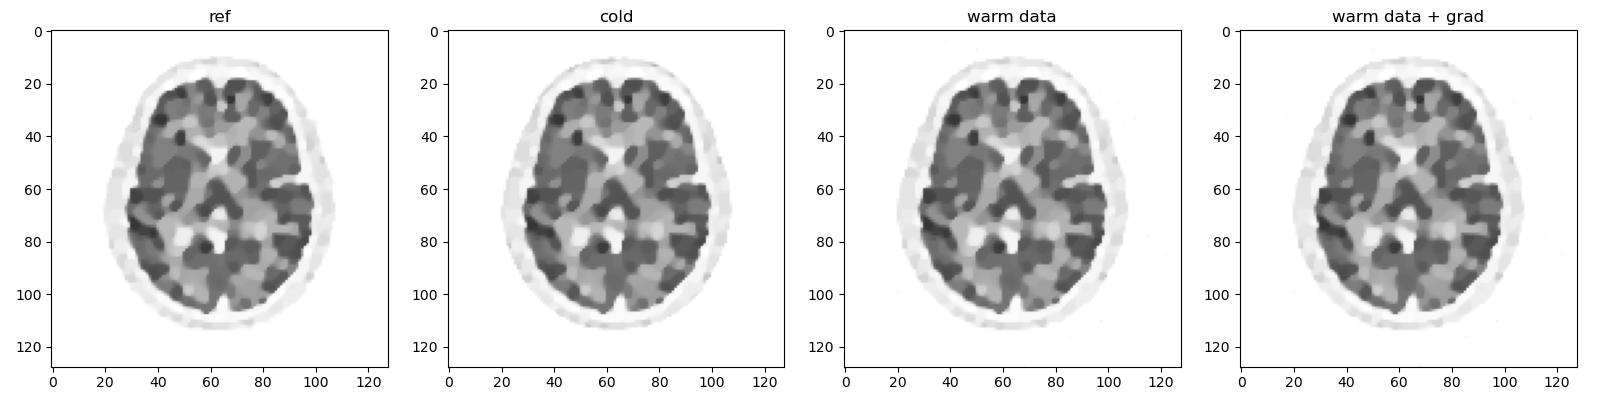
\includegraphics[width=1.0\textwidth]{figs/SPDHG_sino_init.png}
    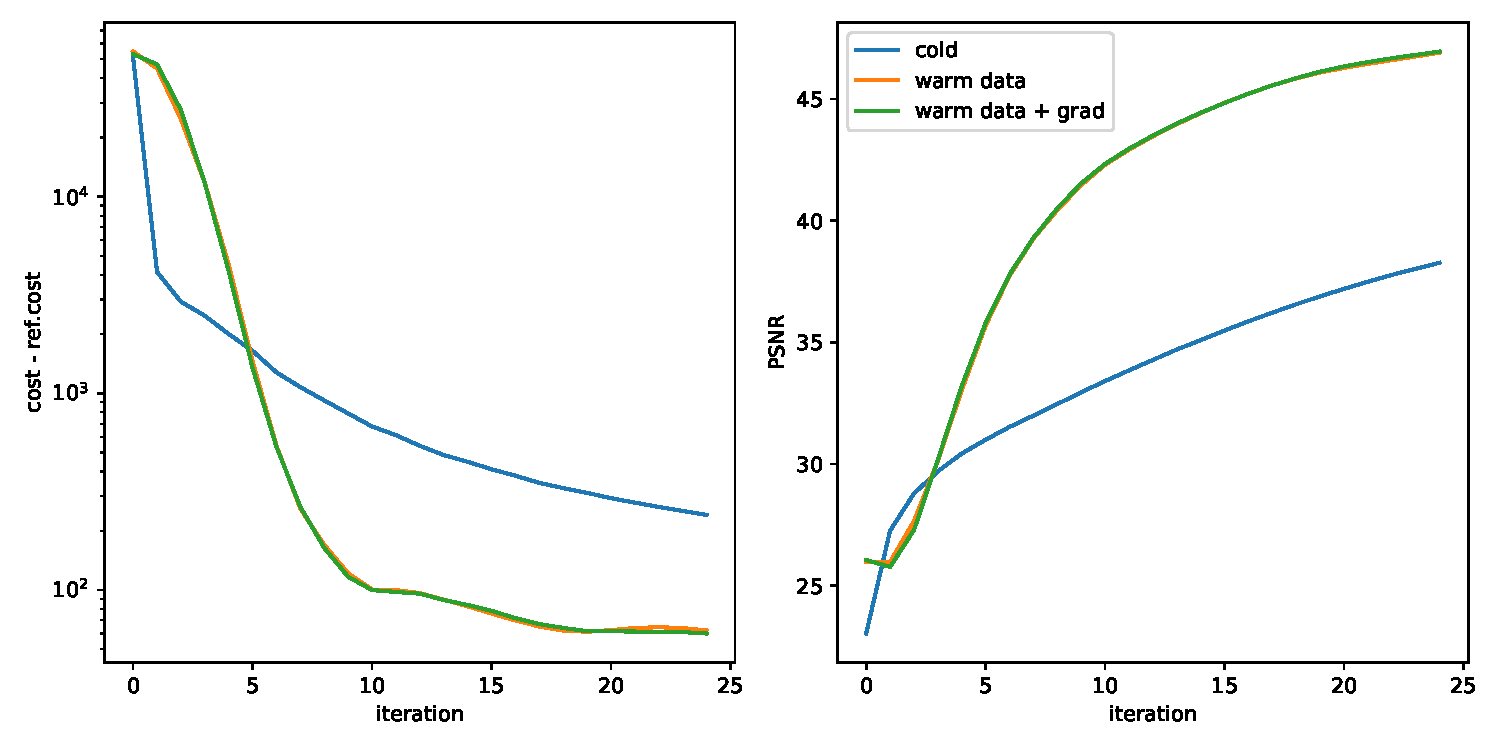
\includegraphics[width=0.8\textwidth]{figs/SPDHG_sino_init_metrics.pdf}
  \caption{$1\cdot10^6$ counts, DTV, $\beta = 0.03$, 112 subsets sinogram SPDHG. ``warm'' start leads to faster convergence in the early iterations.}
  \label{fig:metrics}
\end{figure*}


\begin{figure*}
  \centering
    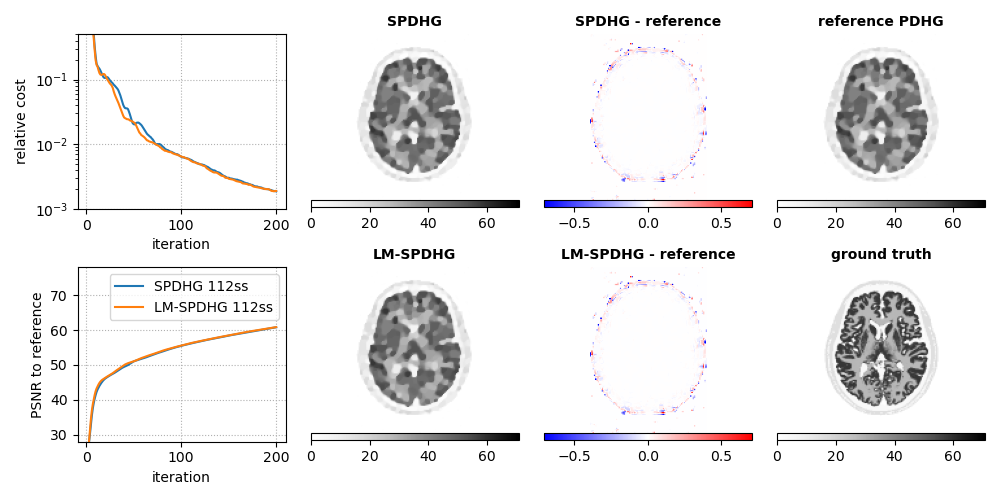
\includegraphics[width=1.0\textwidth]{./figs/brain2d_counts_1.0E+06_seed_1_beta_3.0E-02_prior_TV_niter_ref_20000_fwhm_4.5_4.5_niter_200.png}
    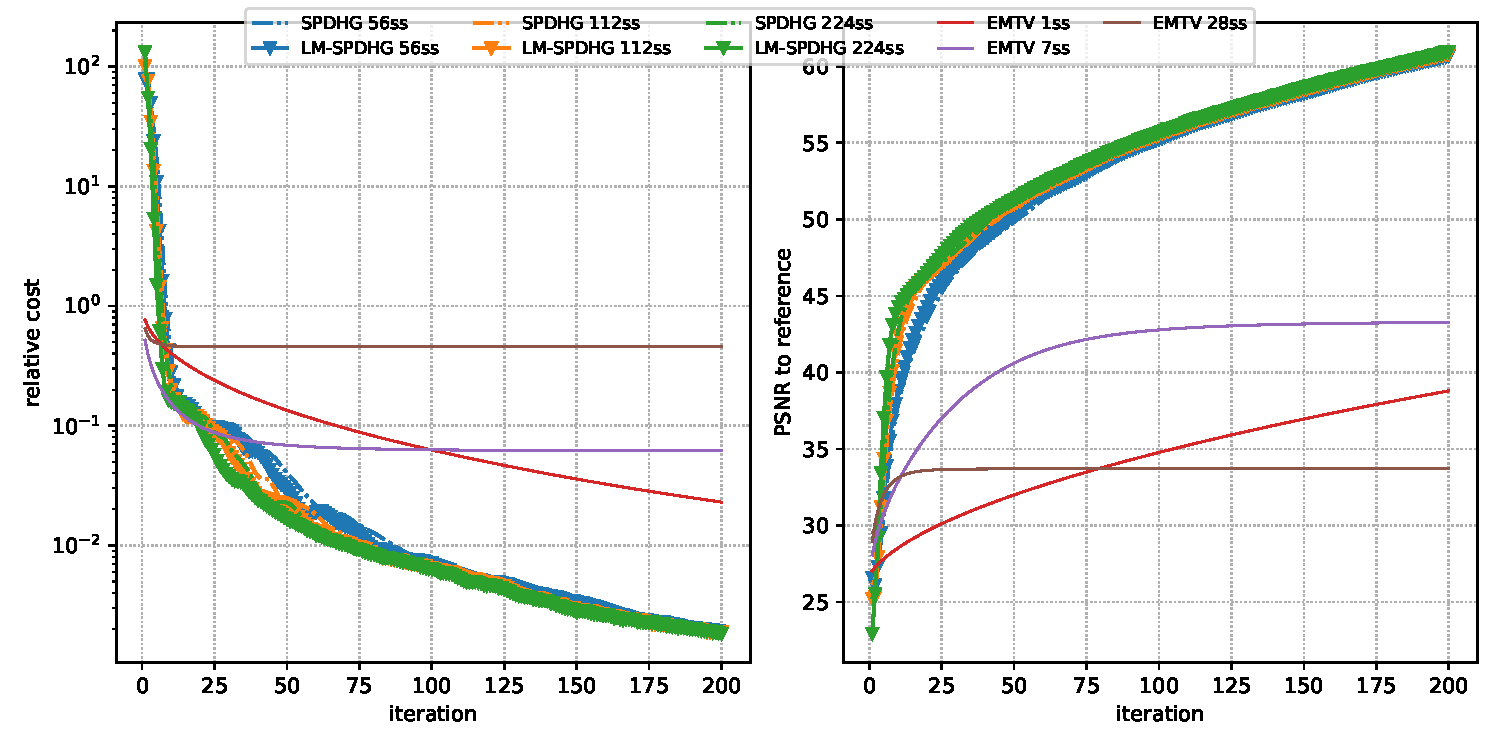
\includegraphics[width=0.8\textwidth]{./figs/brain2d_counts_1.0E+06_seed_1_beta_3.0E-02_prior_TV_niter_ref_20000_fwhm_4.5_4.5_niter_200_metrics.pdf}
  \caption{$1\cdot10^6$ counts, TV, $\beta = 0.03$}
  \label{fig:metrics}
\end{figure*}

\begin{figure*}
  \centering
    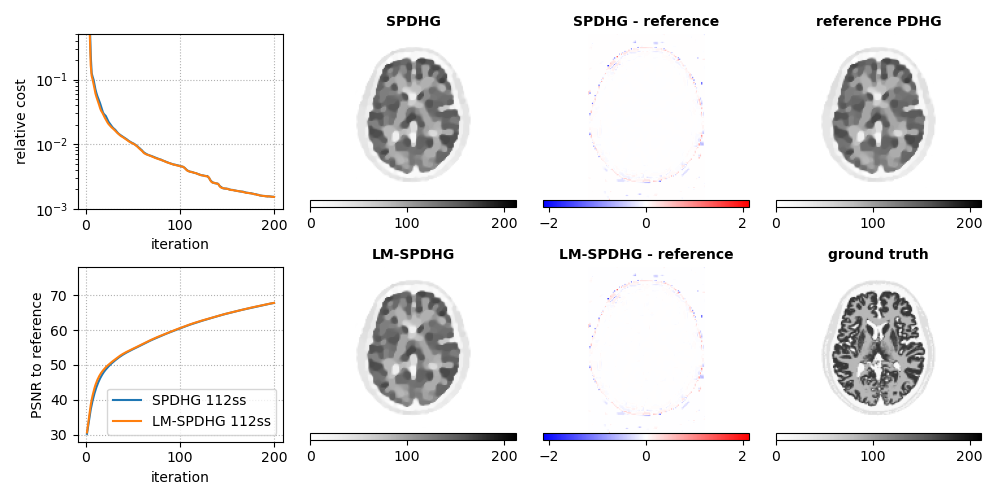
\includegraphics[width=1.0\textwidth]{./figs/brain2d_counts_3.0E+06_seed_1_beta_3.0E-02_prior_TV_niter_ref_20000_fwhm_4.5_4.5_niter_200.png}
    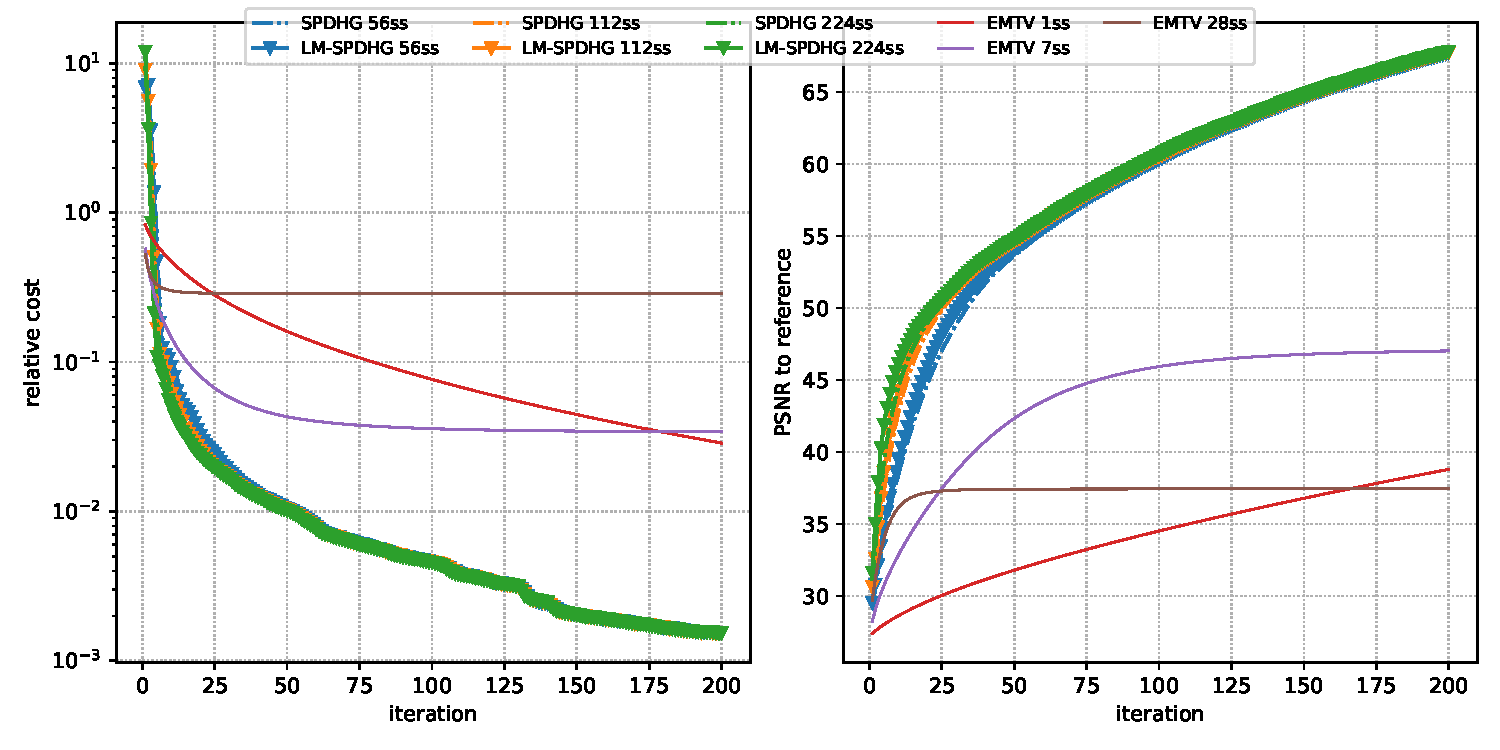
\includegraphics[width=0.8\textwidth]{./figs/brain2d_counts_3.0E+06_seed_1_beta_3.0E-02_prior_TV_niter_ref_20000_fwhm_4.5_4.5_niter_200_metrics.pdf}
  \caption{$3\cdot10^6$ counts, TV, $\beta = 0.03$}
  \label{fig:metrics}
\end{figure*}

\begin{figure*}
  \centering
    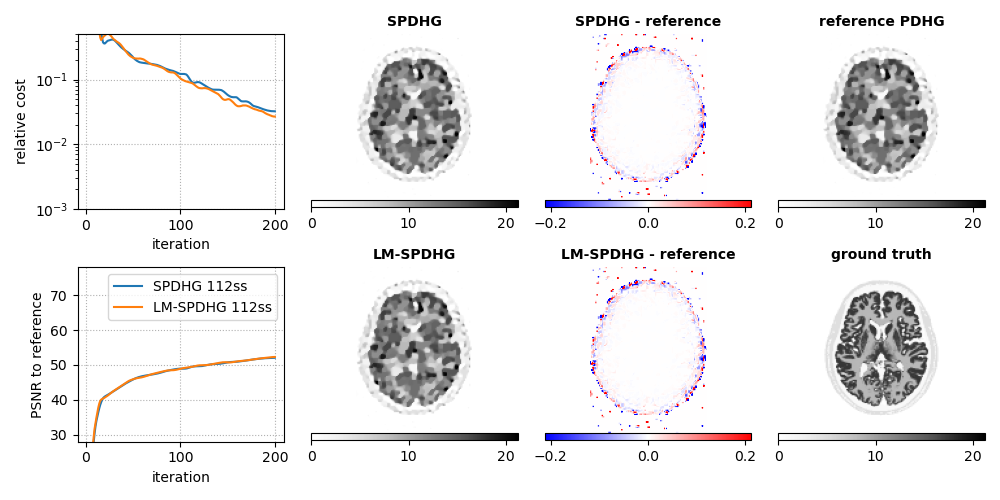
\includegraphics[width=1.0\textwidth]{./figs/brain2d_counts_3.0E+05_seed_1_beta_3.0E-02_prior_TV_niter_ref_20000_fwhm_4.5_4.5_niter_200.png}
    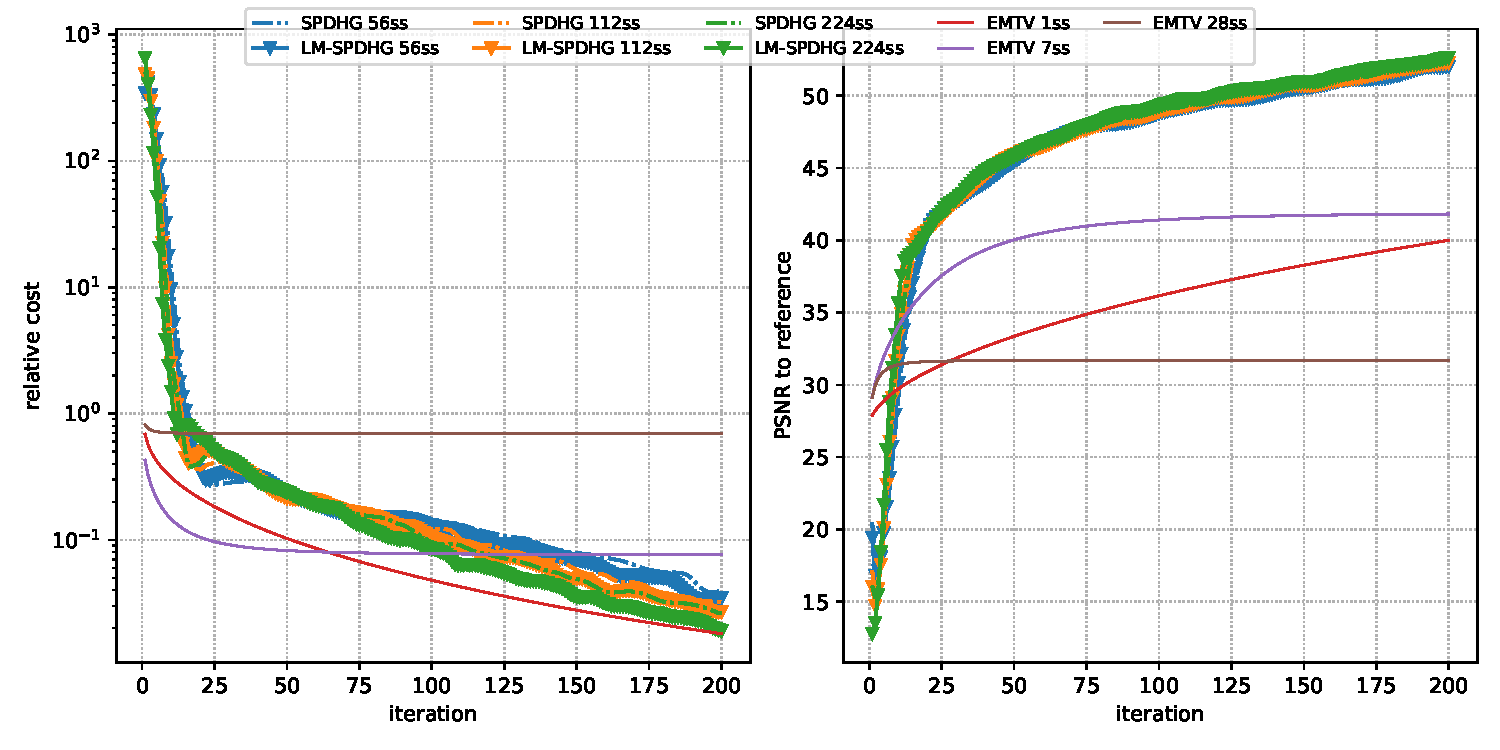
\includegraphics[width=0.8\textwidth]{./figs/brain2d_counts_3.0E+05_seed_1_beta_3.0E-02_prior_TV_niter_ref_20000_fwhm_4.5_4.5_niter_200_metrics.pdf}
  \caption{$3\cdot10^5$ counts, TV, $\beta = 0.03$}
  \label{fig:metrics}
\end{figure*}

\begin{figure*}
  \centering
    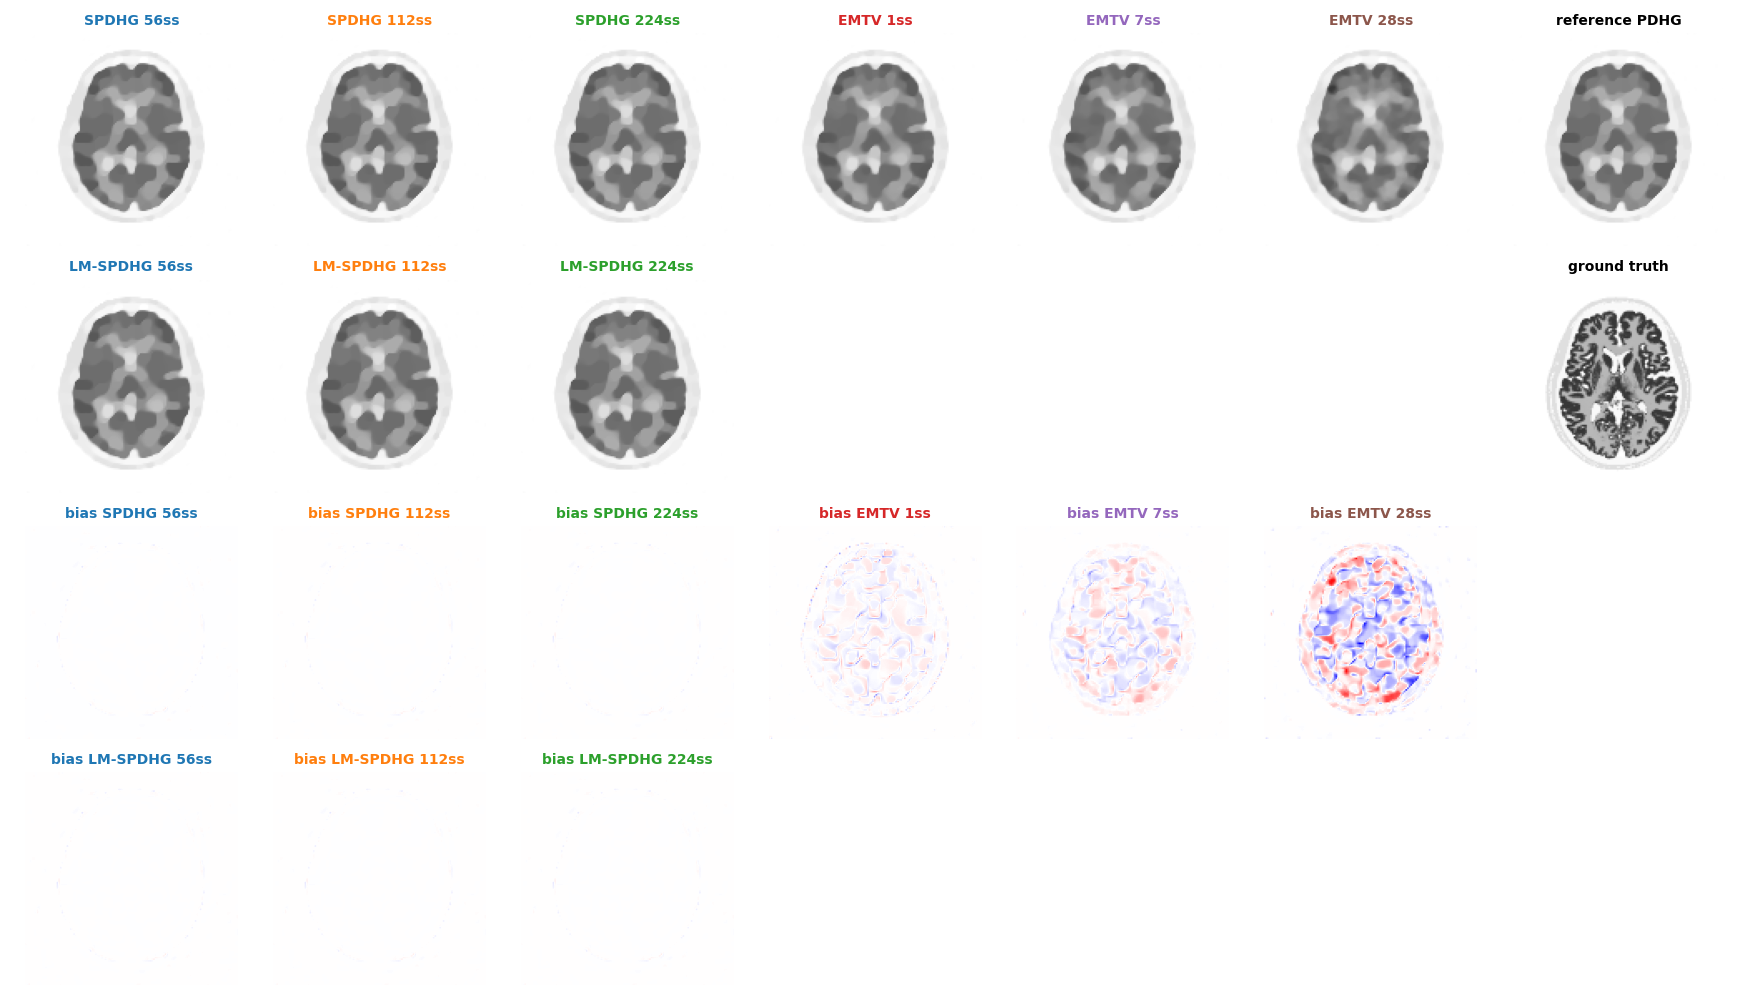
\includegraphics[width=1.0\textwidth]{./figs/brain2d_counts_1.0E+06_seed_1_beta_1.0E-01_prior_TV_niter_ref_20000_fwhm_4.5_4.5_niter_200.png}
    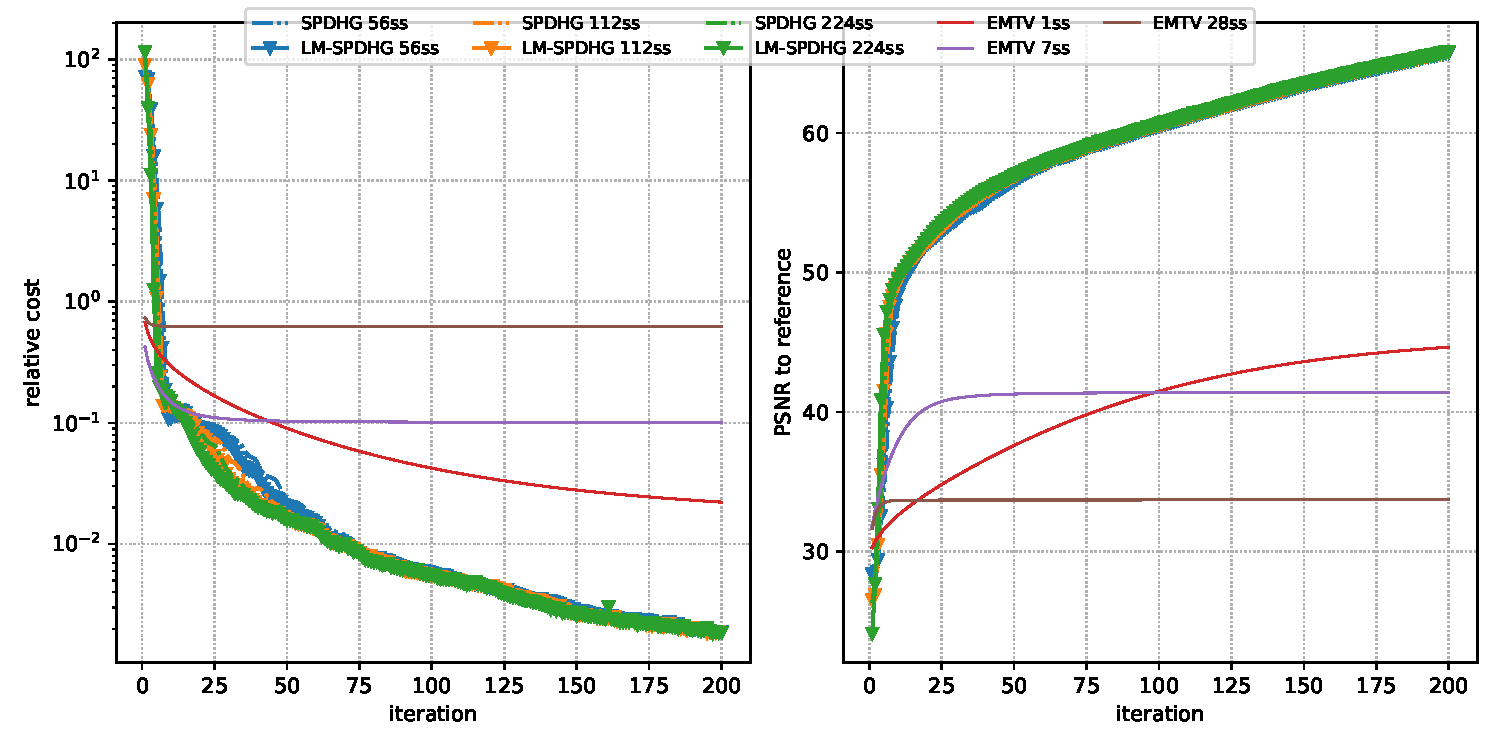
\includegraphics[width=0.8\textwidth]{./figs/brain2d_counts_1.0E+06_seed_1_beta_1.0E-01_prior_TV_niter_ref_20000_fwhm_4.5_4.5_niter_200_metrics.pdf}
  \caption{$1\cdot10^6$ counts, TV, $\beta = 0.1$}
  \label{fig:metrics}
\end{figure*}

\begin{figure*}
  \centering
    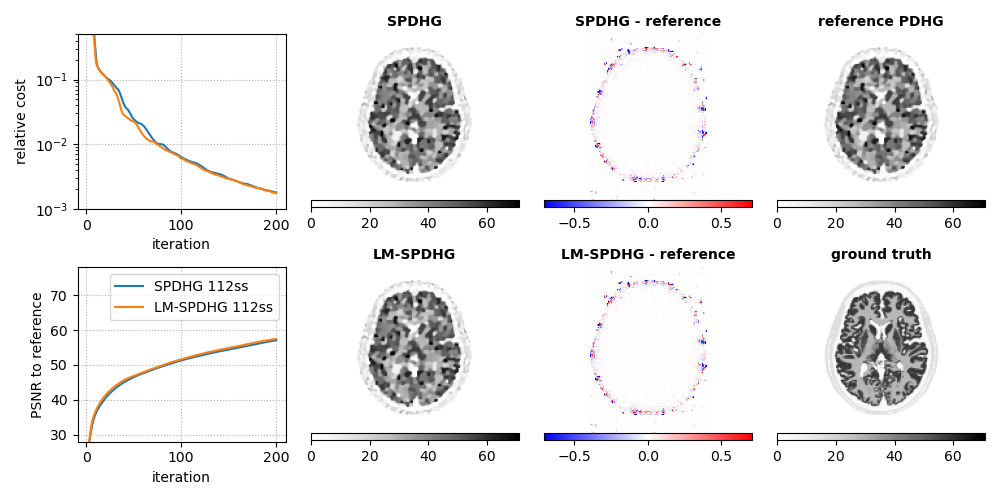
\includegraphics[width=1.0\textwidth]{./figs/brain2d_counts_1.0E+06_seed_1_beta_1.0E-02_prior_TV_niter_ref_20000_fwhm_4.5_4.5_niter_200.png}
    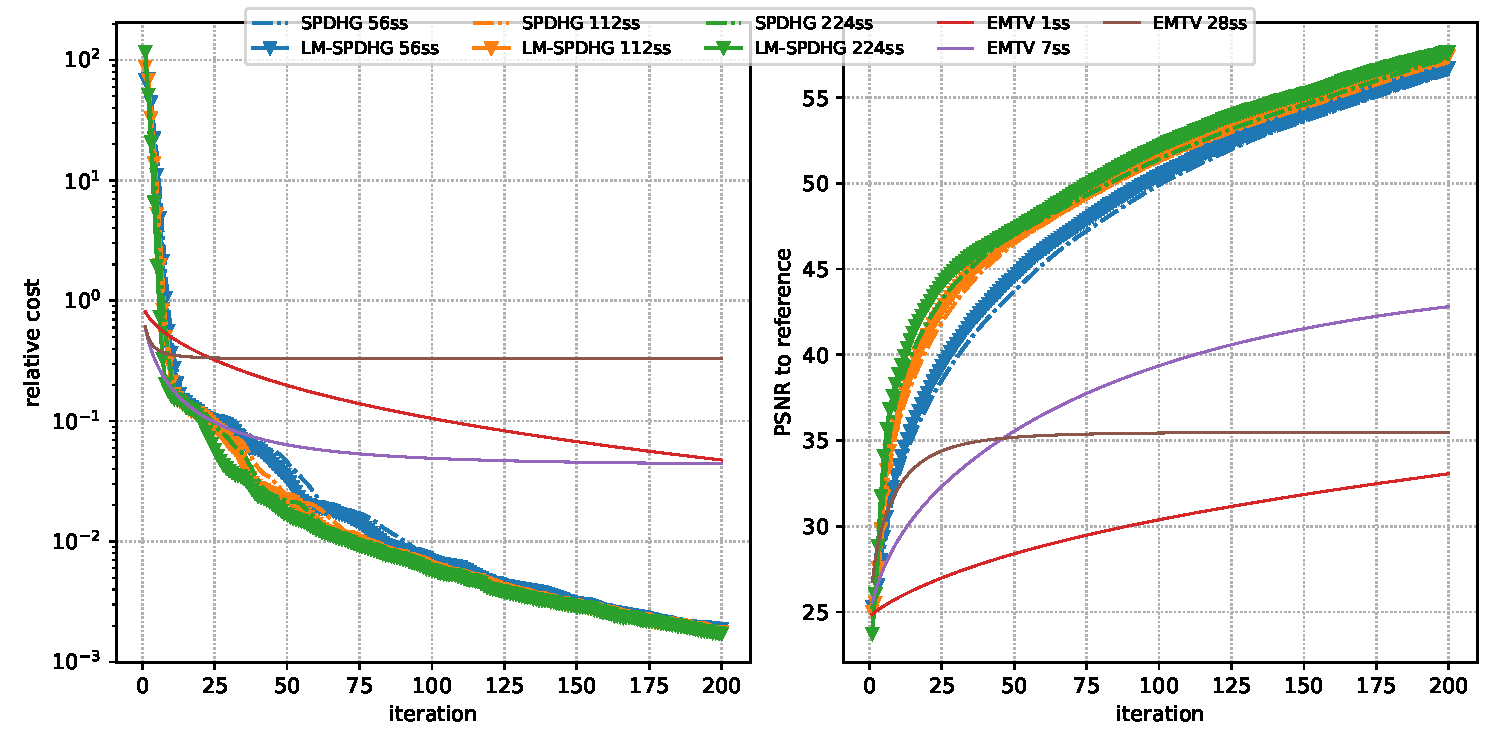
\includegraphics[width=0.8\textwidth]{./figs/brain2d_counts_1.0E+06_seed_1_beta_1.0E-02_prior_TV_niter_ref_20000_fwhm_4.5_4.5_niter_200_metrics.pdf}
  \caption{$1\cdot10^6$ counts, TV, $\beta = 0.01$}
  \label{fig:metrics}
\end{figure*}

\begin{figure*}
  \centering
    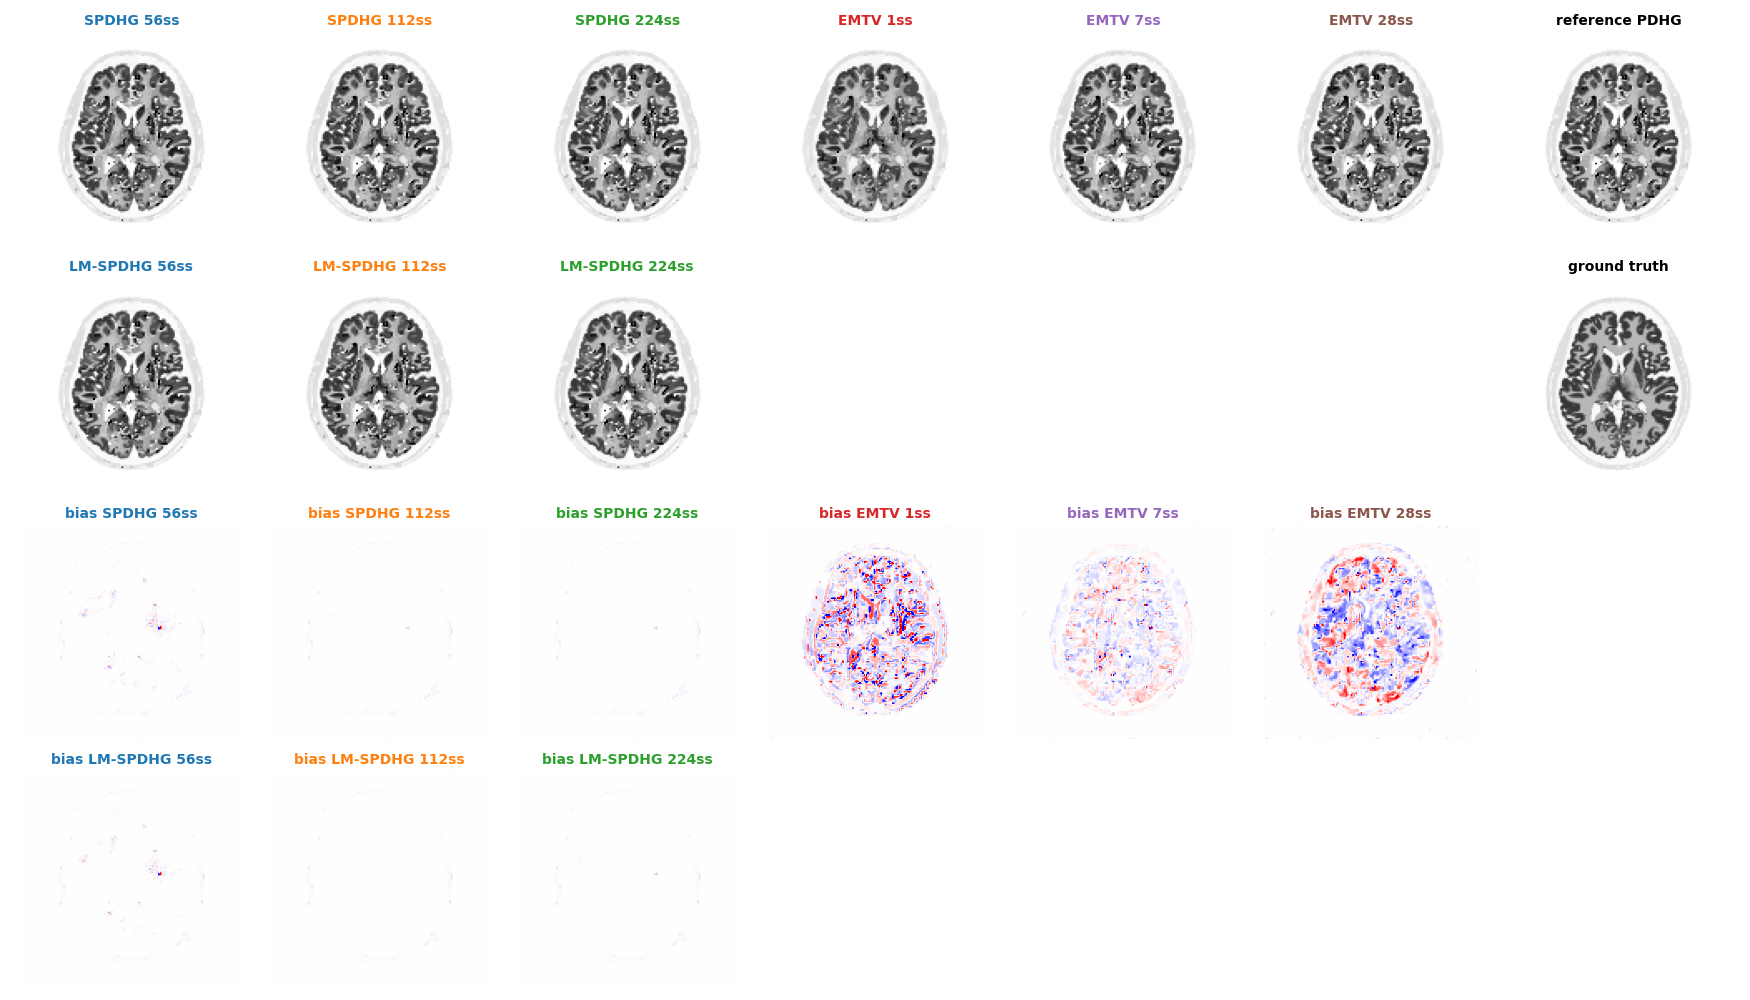
\includegraphics[width=1.0\textwidth]{./figs/brain2d_counts_1.0E+06_seed_1_beta_1.0E-01_prior_DTV_niter_ref_20000_fwhm_4.5_4.5_niter_200.png}
    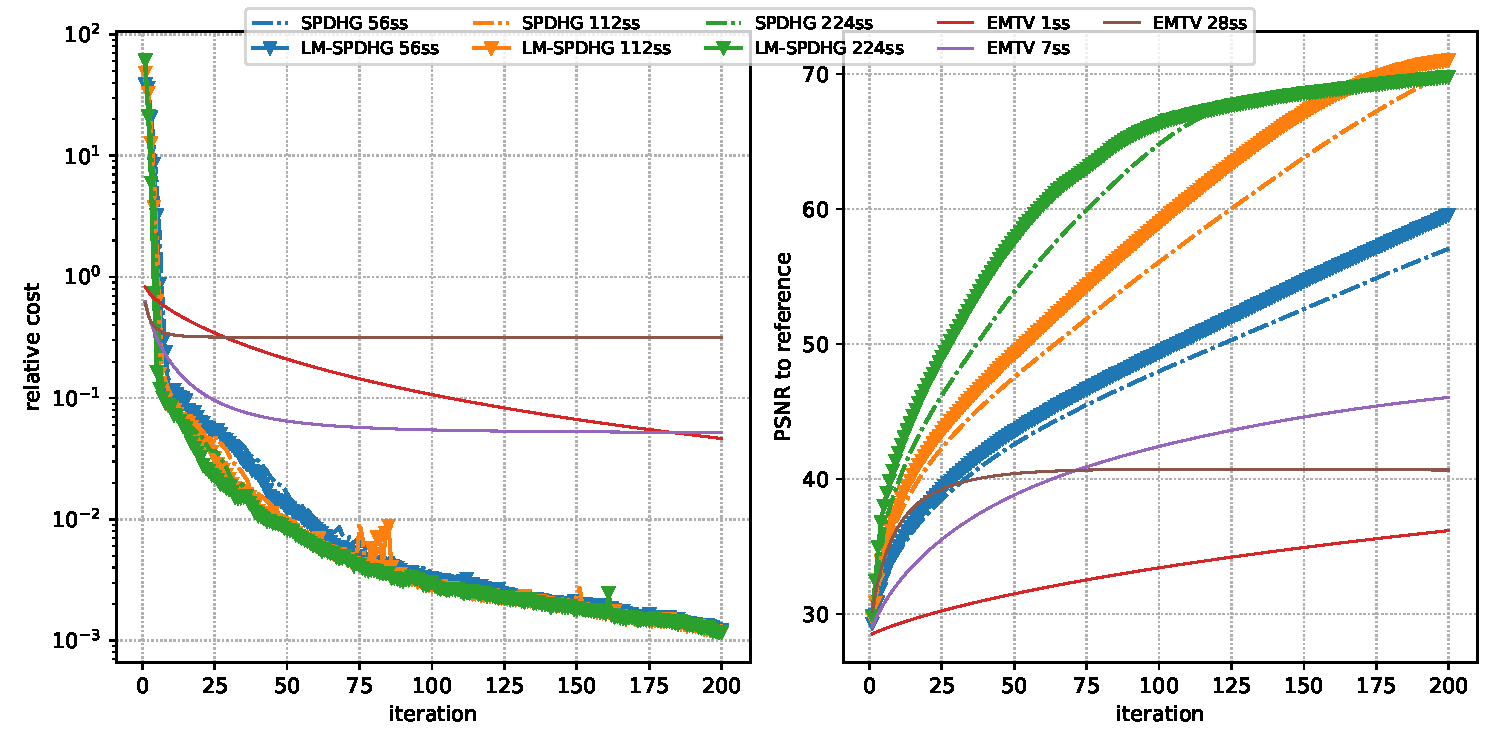
\includegraphics[width=0.8\textwidth]{./figs/brain2d_counts_1.0E+06_seed_1_beta_1.0E-01_prior_DTV_niter_ref_20000_fwhm_4.5_4.5_niter_200_metrics.pdf}
  \caption{$1\cdot10^6$ counts, DTV, $\beta = 0.1$}
  \label{fig:metrics}
\end{figure*}
